\documentclass[UTF8]{ctexart}
\usepackage[paper=a4paper,dvips,top=2.5cm,left=2.8cm,right=2.8cm,foot=1cm,bottom=3.2cm]{geometry}
\usepackage{fancyhdr}
\usepackage{indentfirst}
\usepackage{enumerate}
\usepackage{clrscode}
\usepackage{listings}
\usepackage{amsmath}
\usepackage{amstext}
 \thispagestyle{empty} 
\lstset{language=Matlab}%代码语言使用的是matlab
\lstset{breaklines}%自动将长的代码行换行排版
\lstset{extendedchars=false}%解决代码跨页时,章节标题,页眉等汉字不显示的问题
\usepackage{graphicx}
\usepackage[colorlinks,linkcolor=blue,urlcolor = blue]{hyperref}
\DeclareGraphicsExtensions{.eps,.ps,.jpg,.bmp}
\pagestyle{plain}
\begin{document}
\par 尊敬的吴老师,您好
\newline 
\par 首先有个坏消息:我的复杂网络暑期课程申请没有通过,被拒了。。
\newline 
\par
在最近的一段时间里,我实现了预测转发链长度的代码。转发链长度预测是在已有的微博关系网络和LIS模型下,预测一条微博的转发用户数量。具体的,假设一条微博$m$从用户$u$开始传播,用户$u$的近邻$v_{i}$接收到微博$m$后,转发此条微博的概率为
\begin{equation}
1-exp(- \lambda I_{u}^{T}S_{v_{i}})
\end{equation}
其中$I_{u}$和$S_{v_{i}}$分别为用户$u$的influence向量和用户$v_{i}$的susceptibility向量。我们使用轮盘赌方法来决定用户$v_{i}$是否转发了此条微博,如果转发了,则将用户$v_{i}$压人队列。考察完用户$u$的所有近邻后,依次取出队列中的用户进行考察,直至队列为空。在此过程中被激活的用户数量则为微博$m$的转发链长度。
\par 对微博数量为$n$的test集来说,经过上述的预测过程后,记录每一转发链长度对应的微博数量,得到以转发链长度为下标的向量$A$。同样的,根据真实的数据得到向量$B$。经过平滑处理后,最后我们利用mean absolute percentage error(MAPE)来评估预测情况。MAPE的计算公式为
\begin{equation}
M = \frac{1}{n}\sum_{t=1}^{n}\left | \frac{A_{t}-F_{t} }{A_{t}}\right |
\end{equation}
其中$A_{t}$是实际值,$F_{t}$是预测值。
\par 实验测试所用的数据集包含199408个用户、972340条连边、395852条微博。实验结果如图$1$所示,结果并不好。真实数据在转发链长度为2处有一个波峰,而预测结果的波峰在1处。同时,MAPE值为1.27,比论文中的结果0.140大了一个数量级,原因暂时还不清楚。
\begin{figure}[h!]
    \centering
    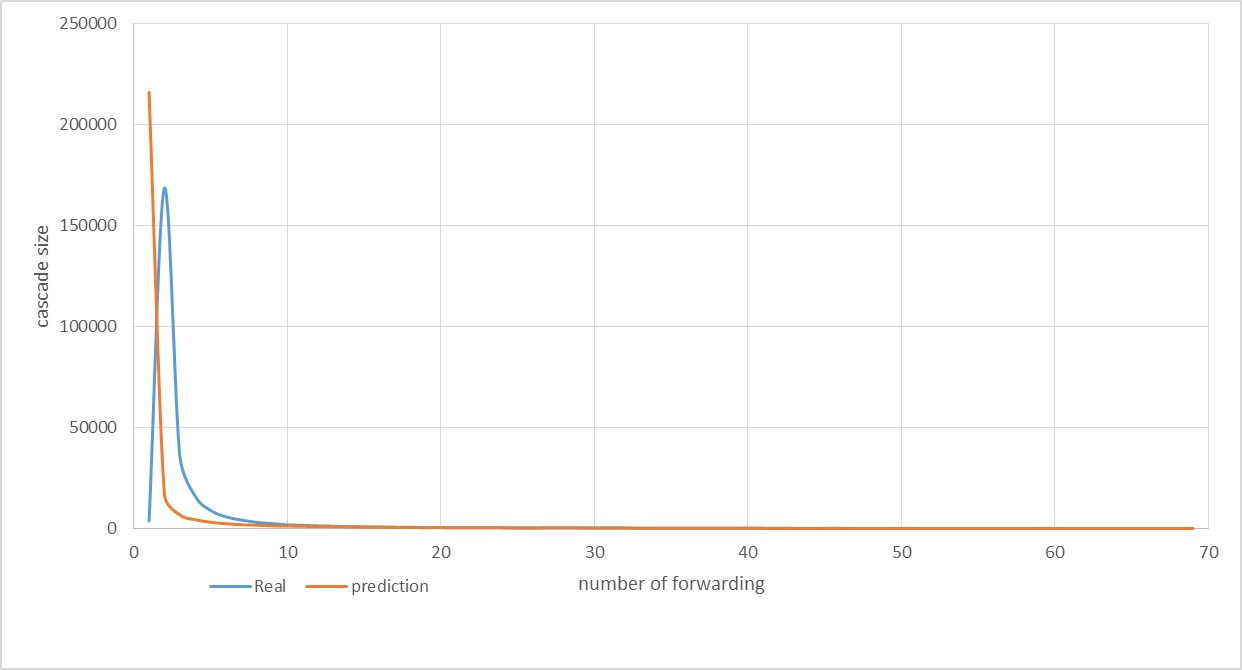
\includegraphics[width=12cm]{cascade.jpg}
    \caption{预测结果}
    \label{fig-sample}
\end{figure}
\par 另外,我读了其他几篇有关微博转发预测的论文,他们解决问题的角度或在于对用户之间的连边权值建模来预测,或结合微博的具体消息内容来预测。
\newline
\par \rightline{学生王超民,2016年6月20日}
\end{document}
